% Candidate-only evidence; root decides the final insertion point.
\subsection{行和缓存候选的双版本数值证据}
\label{sec:row-cache-evidence}
本节对应候选 RTL 内容摘要 \code{1e3fab94b7b2}\ldots，包含 26 项生产 RTL 文件；父提交为 \code{f028ec5}。
来源为 \code{docs/evidence/20260930/row_cache/}，属于新的本地功能验收，不能移用父提交 CI 的通过结论。
归档中的 Verilator 5.020 与运行时标识为 5.49 的开发版，分别完成相同的五种加载器几何和七种归约器几何。
每个版本的 16,150 个加载事务步与 1,430,848 个归约输入样本按各自单位列示，不相加为覆盖率。
5.020 的附加复验只包括这两项，不能据此声称该工具本地重跑了全部 22 个 bench。

\begin{figure}[htbp]\centering
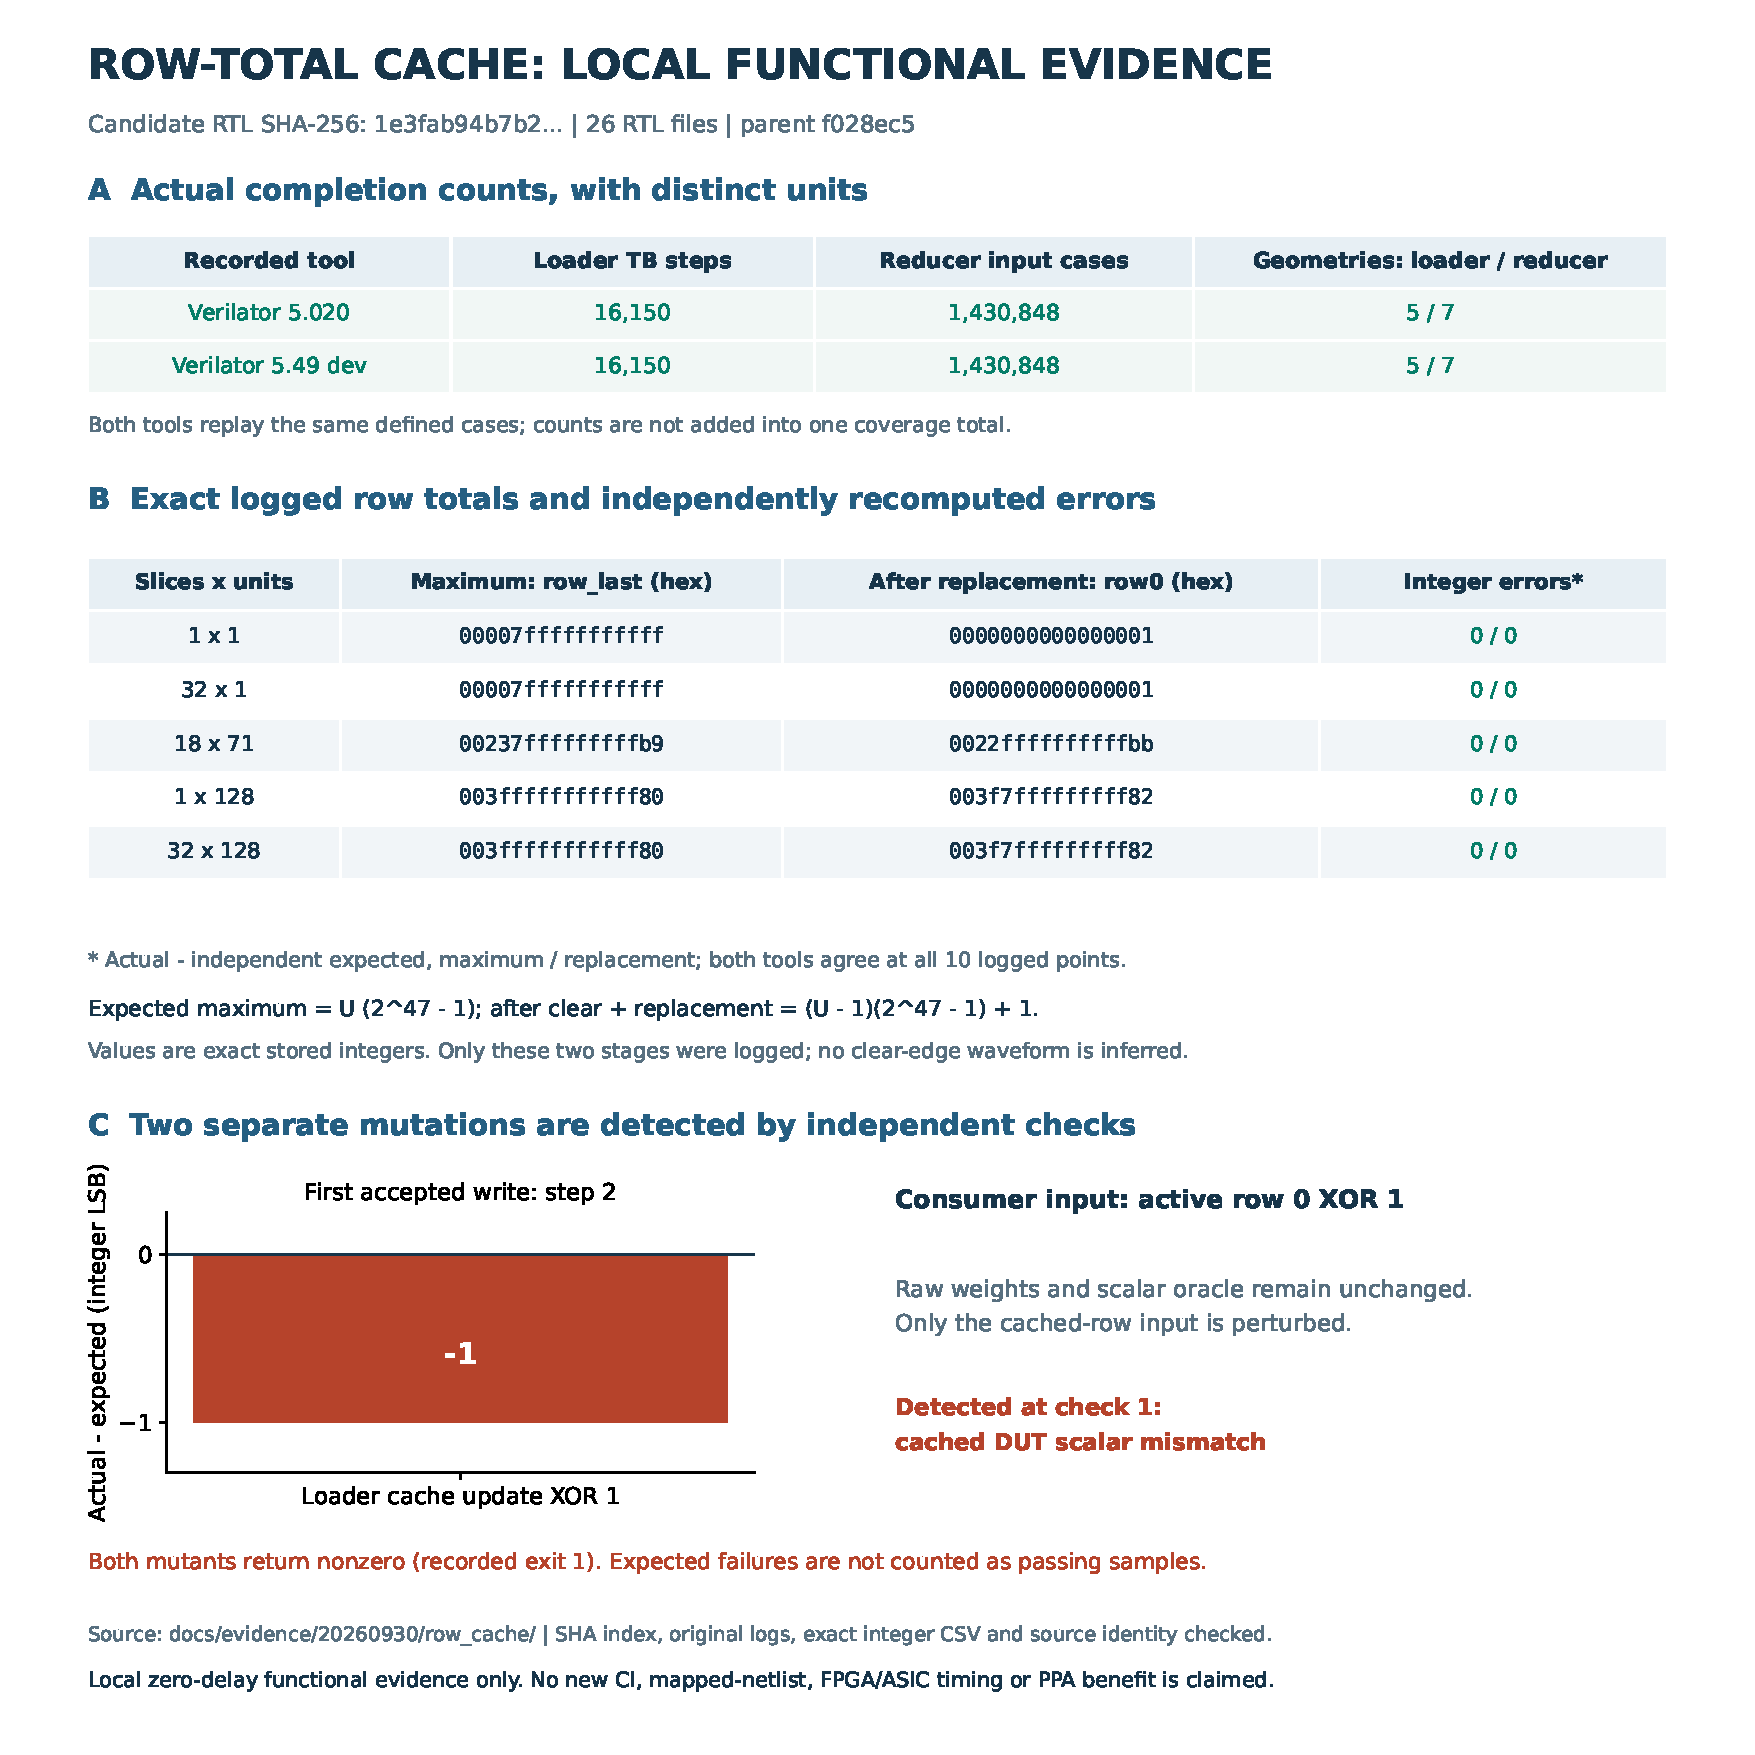
\includegraphics[width=\textwidth]{figures/41_row_cache_evidence.pdf}
\caption{候选行和缓存的真实日志证据。上表为双版本完成计数；中表为五种几何在最大装载和 clear 后替换两个已记录阶段的精确十六进制整数，独立整数公式的误差均为零。下方展示两个分别注入的错误被检出；没有由完成标记推造波形，也没有将功能通过解释为 PPA 收益。}
\label{fig:row-cache-evidence}
\end{figure}

最大装载先把整张表写为 \(W_{\max}=2^{47}-1\)，故每个含 \(U\) 项的物理行应为 \(U W_{\max}\)。
\code{clear_load} 清除完整性位图，保留权重与行和；随后将行 0 的一个旧最大权重替换为 1，
独立期望成为 \((U-1)W_{\max}+1\)。图\ref{fig:row-cache-evidence}分别保留原日志的 \code{row_last} 与 \code{row0} 标签。
制图器以 Python 任意精度整数重新计算，不把超过 \(2^{53}\) 的行和先转为浮点数再判断相等。
全部十个阶段观测在两个版本原始日志中逐条匹配；归档没有单独记录 clear 当拍的数值，因而不额外绘制该时刻。

两个负控分别检查生产者和消费者。
第一项只翻转行和写回结果的最低位，在首次接受写的第 2 步出现实际值相对独立期望少 1，加载器检查立即失败。
第二项只翻转活动行 0 的缓存输入最低位，原始权重、未缓存实现、旧公式和 scalar oracle 都不变；
第 1 个比较样本触发 \code{cached DUT scalar mismatch}。
后者排除了“缓存输入被忽略而仍通过普通数值回归”的假阳性；它不是新功能正常输出的样本。

可复现入口为 \code{audit_figures/make_row_cache_evidence.py}，来源清单为 \code{audit_figures/41_source_hashes.json}。
脚本校验归档 SHA、26 项 RTL 摘要、完成计数、十个实测值以及两份负控的失败日志与源文件摘要。
这些结果说明行和维护与消费在所测功能条件下符合独立判据；缓存候选的实际资源、物理建立/保持时序及 ASIC 目标频率仍应由同一候选的后续综合和实现报告单独判定。
